%%*****************************************************************************
%% $Id$
%%*****************************************************************************
%%
%% Copyright (C) 2005-2009 The ExTeX Group and individual authors listed below
%%
%% This library is free software; you can redistribute it and/or modify it
%% under the terms of the GNU Lesser General Public License as published by the
%% Free Software Foundation; either version 2.1 of the License, or (at your
%% option) any later version.
%%
%% This library is distributed in the hope that it will be useful, but WITHOUT
%% ANY WARRANTY; without even the implied warranty of MERCHANTABILITY or
%% FITNESS FOR A PARTICULAR PURPOSE. See the GNU Lesser General Public License
%% for more details.
%%
%% You should have received a copy of the GNU Lesser General Public License
%% along with this library; if not, write to the Free Software Foundation,
%% Inc., 59 Temple Place, Suite 330, Boston, MA 02111-1307 USA
%%
%%*****************************************************************************
%% @author Gerd Neugebauer
%%-----------------------------------------------------------------------------
\chapter{Prerequisites}

\section{Java}

You need to have \+Java+ 6 or later installed on your system. You can
get Java for a several systems directly from \url{java.sun.com}.
Download and install it according to the installation instructions for
your environment.

To check that you have an appropriate Java on your path you can use
the command \texttt{java} with the argument \texttt{-version}. This
can be seen in the following listing:

\lstset{morecomment=[l]{\#}}%
\begin{lstlisting}{morecomment=[l][keywordstyle]{>}}
# java -version
java version "1.6.0_15"
Java(TM) SE Runtime Environment (build 1.6.0_15-b03)
Java HotSpot(TM) Client VM (build 14.1-b02, mixed mode, sharing)
#
\end{lstlisting}

Other Java implementations are currently not supported. They might
work, but the last time we checked it, \+GCJ+ didn't suffice. We would
be happy to have someone working on a compatibility layer for a other
Java implementations.


\section{TEXMF}\index{TEXMF|(}

If you want to use more than the pure \ExTeX\ engine, fonts and macros
can be inherited from a texmf tree\index{texmf}. \ExTeX\ itself does
not contain a full texmf tree. It comes just with some rudimentary
files necessary for testing. Thus you should have installed a texmf
tree, e.g. from a \TeX Live\index{TeXlive@\TeX Live} installation.
This can be found on the \href{http://www.ctan.org}{Comprehensive
  \TeX\ Archive Network (CTAN)}\index{CTAN}.

There is no need to install the texmf tree in a special place. You
have to tell \ExTeX\ anyhow where it can be found. It is even possible
to work with several texmf trees.

One requirement for the texmf trees is that they have a file database
(\File{ls-R}). \ExTeX\ can be configured to work without it, but then
\ExTeX\ is deadly slow. Thus you do not really want to try this
alternative.

To use your texmf tree you should create a configuration file in your
home directory. On a Unix\index{Unix} system the home directory is
stored the environment variable
\verb|$HOME|\index{HOME@\texttt{\$HOME}}. On a \+Windows+ system the
home directory is usually located under \verb|C:\WINDOWS\Profiles\|.
The configuration file must have the name \File{.extex} (a little
intelligence test under \+Windows+;-). It contains one line of the
following form

\begin{lstlisting}{}
texmf.path=/usr/lib/texmf
\end{lstlisting}

The value should point to the location of the texmf tree. If you have
several TEXMF trees which need to be used you can put them into this
attribute by separating them by a platform-specific separator. This
separator is a colon (\verb|:|) under \+Unix+ and a semicolon
(\verb|;|) under \+Windows+. \index{TEXMF|)}

\section{Subversion Client}\index{Subversion|(}

\ExTeX{} uses Subversion (\url{http://subversion.tigris.org/}) as
revision control system.\footnote{\ExTeX{} has used CVS\index{CVS} in
  the beginning. Thus references to CVS might be left over.} Thus you
need a Subversion client installed on your machine. In the simplest
case this is the client integrated into the IDE Eclipse (see
section~\ref{sec:eclipse.plugins}), or the command line version of
\texttt{svn}.

On Unix systems the Subversion command line client might be available
in the form of the used package system. Otherwise download it from the
Subversion site and install it according to the instructions.

On Windows \+TortoiseSNV+ (\url{http://tortoisesvn.tigris.org/}) can
be used. It is an integration into the Explorer which simplifies the
access to a subversion repository without a separate client.
\index{Subversion|)}


\section{Maven}\index{Maven|(}

The \+build system+ is based on Maven~2 (\url{http://maven.apache.org/}).
Thus Maven~2 needs to be installed. To install Maven 

\begin{itemize}
\item load it down from its download site -- or a mirror close by,
\item unpack the archive to a destination directory,
\item define an environment variable
  \texttt{MAVEN\_HOME}\index{MAVEN\_HOME@\texttt{MAVEN\_HOME}} to
  point to the unpacked directory, and
\item put \texttt{\$MAVEN\_HOME/bin} onto the path.
\end{itemize}

 \index{Maven|)}


\section{Ant}\index{Ant|(}

Ant is used at some places in the old \+build system+. Thus it might
be necessary to have Ant installed and on the path for special tasks.
\index{Ant|)}


\section{Perl}\index{Perl|(}

Perl (\url{http://www.perl.org/}) is used to create the web site. Thus
it has to be installed for this purpose. For the usual development it
is not necesary to have Perl installed. \index{Perl|)}


\section{A Command Line Interpreter}\index{Shell|(}

For several tasks it is convenient to have a command line interpreter
at hand. On \+Unix+ this can be the (bourne\index{bourne shell},
\+bash+, korn\index{korn shell}\ldots) shell. On \+Windows+ we
recommend the \+Cygwin+ suite (http://cygwin.com/) which contains
bash.  \index{Shell|)}

\section{User Account at Berlios}\index{Berlios|(}

To commit changes to the repository you have to be enlisted as a
developer for \ExTeX. A first requirement for this is an account at
Berlios -- the hosting site. If you just want to read the sources then
you can use anonymous access.

To register at Berios use the page \url{http://developer.berlios.de/}
and select the item \menu{} on the upper left side. You will find
yourself in the registration page as shown in
figure~\ref{fig:berlios-register}. You will find your way through
easily.
\begin{figure}[htbp]
  \centering  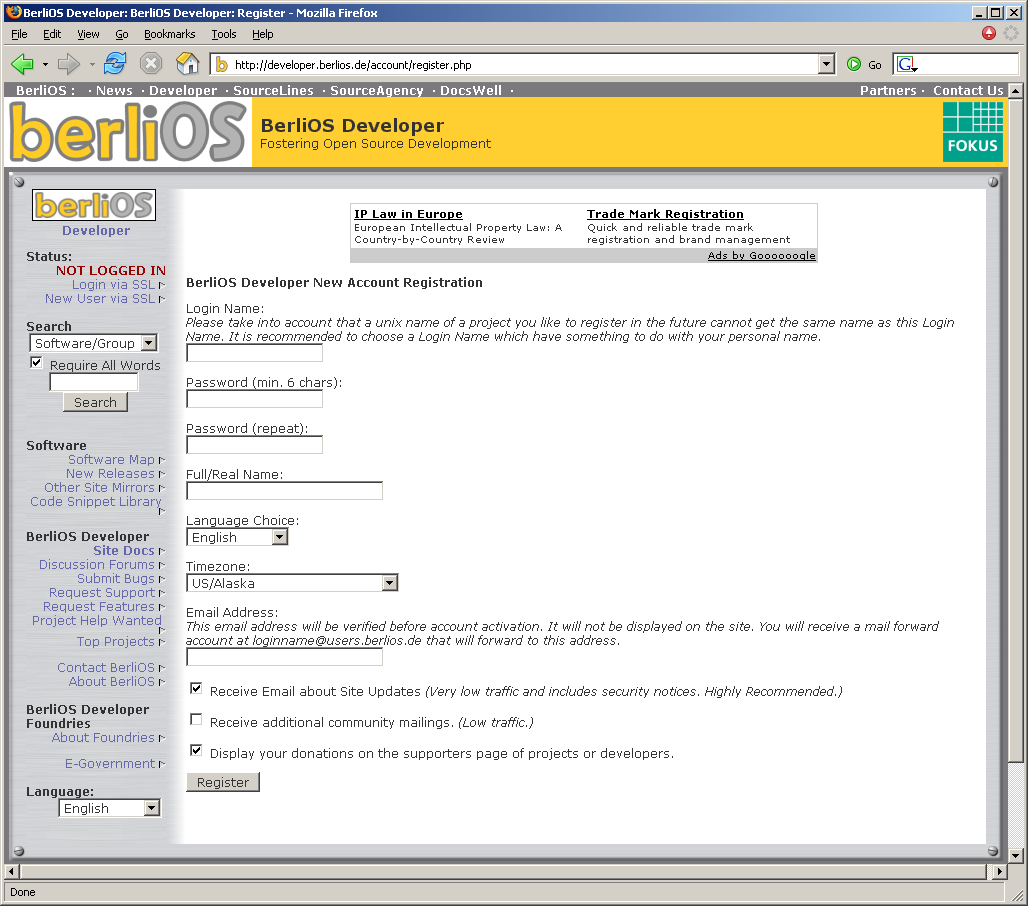
\includegraphics[scale=.33]{image/berlios-register}
  \caption{New Account at Berlios}\index{Berlios!account}\label{fig:berlios-register}
\end{figure}

When you have an account at Berlios you might be added to the
developers list of \ExTeX. This as to be done by one of the admins of
\ExTeX. Contact us via the developer mailing list \index{Berlios|)}

